\chapter{Android y Google App Engine.}\label{cap:androidYGAE}
\markboth{CAPÍTULO \ref{cap:androidYGAE}. ANDROID Y GOOGLE APP ENGINE.}{}

En este capítulo vamos a explicar más detenidamente las dos principales plataformas usadas durante el proyecto, Android en la parte móvil y Google App Engine en la parte de las aplicaciones web. 

\section{Android}\label{cap:android}

\subsection{Introducción.}

Android es un sistema operativo basado en Linux, libre y multiplataforma. Inicialmente empezó como un sistema operativo solo para móviles pero con el tiempo ya podemos encontrarlo en móviles, tablets, pc, neveras, relojes, cámaras de fotos y una gran cantidad de aparatos.

En el proyecto lo usaremos para diseñar y desarrollar una aplicación móvil, con la que poder firmar digitálmente un texto leido previamente mediante un lector de códigos QR.

Android es propiedad de Google actualmente y es el encargado de dar soporte y ayudar a los desarrolladores. Esta función la realiza muy bien, dando una muy buena API y una gran documentación. Podemos encontrar toda la información que podemos necesitar para desarrollar una aplicación en la siguiente web, \url{http://developer.android.com/index.html}. En la anterior web podemos encontrar la documentación de la API, consejos de diseño para que la aplicación tenga un aspecto bonito a la vez que usable, todas las novedades incluidas en las versiones nuevas del sistema operativo, etc.

\subsection{Arquitectura de la plataforma Android.}

Como hemos dicho anteriormente Android es una plataforma que engloba desde el sistema operativo, al software intermedio que comunica el sistema operativo y las aplicaciones, llamado en inglés middleware y las posibilidad de hacer funcionar las aplicaciones en la plataforma elegida, ya sea un telefono, un tablet o cualquier aparato con Android.

Para los desarrolladores Android proporciona dos kit de desarrollo, uno que usa la tecnología Java (SDK), el que hemos usado en el proyecto y otro que da la posibilidad de programar a más bajo nivel (NDK), este último desarrollado en C++.

El SDK de Android proporciona ayuda para las siguientes características, un navegador basado en WebKit, graficos optimizados en 2D, gráficos en 3D basados en OpenGL ES 1.0 con aceleración gráfica, una base de datos para almacenar datos que necesitemos, llamada SQLite, soporte para ficheros gráficos (JPG, PNG, GIF, etc), vídeo (MPEG4, H.264) y audio (MP3, AAC), telefonía GSM, tecnologías inalámbricas como son Bluetooth, 3G, Wifi, uso de la cámara, GPS, brújulas, etc. Además de todo esto, proporciona ayuda en la reutilización y remplazo de componentes, una máquina virtual optimizada para dispositivos móviles llamada Dalvik y un emulador donde poder probar la aplicación antes del lanzamiento sin tener que poseer un terminal Android. 

\begin{figure}
  \centering
    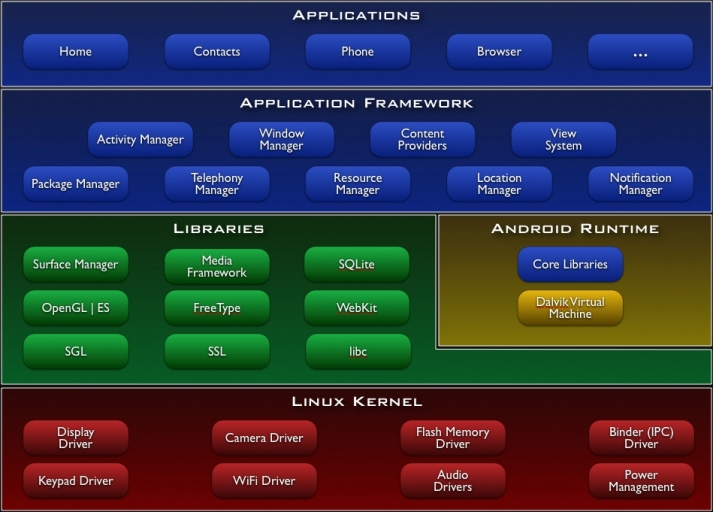
\includegraphics[scale=0.6]{./Android/imagenes/arquitecturaAndroid.jpg}
  \caption{Arquitectura de Android.}
  \label{fig:arquitecturaAndroid}
\end{figure} 

La arquitectura la podemos ver en la figura~\ref{fig:arquitecturaAndroid}. En la imagen podemos observar las cinco capas principales en las que se divide Android.
\begin{itemize}

\item \textbf{Applications:} en esta capa están todas las aplicaciones que nos proporciona el sistema operativo de base, como pueden ser la lista de contactos, un gestor de SMS, el navegador, el lanzador de aplicaciones, todas las aplicaciones de servicios de Google, como pueden ser Gmail, Google Maps, Google Calendar, Google Reader.   

\item \textbf{Application framework:} en esta capa está todo lo relacionado con los manejadores de activitys, llamadas de telefono, controladores de vistas. Es una capa que hay intermedia para manejo de hardware, con la que se pueden controlar tanto las notificaciones, como servicios que se ejucutan en segundo plano, etc. Los desarrolladores tienen el mismo acceso mediante esta capa de la API a todos los servicios que las aplicaciones nativas que proporciona el sistema el operativo. 

\item \textbf{Libraries:} como su nombre indica en esta capa están todas las librerías que el sistema operativo necesita, para manejo de archivos multimedia, manejo de gráficos 3D, renderizado web, etc.

\begin{itemize}
	\item \textbf{System C library:} una implementación del estandar C, optimizada para funcionar en sistemas móviles para las funciones del kernell de linux.
	\item \textbf{Media Libraries:} librerías basadas en PacketVideo's OpenCORE para grabación y reproducción de formatos de audio y video mas populares del momento como MP3, H.264, JPG o PNG.

	\item \textbf{Surface Manager:} librería para manejo de graficos 2D y 3D para varias aplicaciones.

	\item \textbf{LibWebCore:} motor de renderizado para navegadores embebidos de páginas web.

	\item \textbf{SGL:} motor para renderizado 2D.

	\item \textbf{3D libraries:} librería que implementa la API de OpenGL ES 1.0, que proporciona aceleración 3D por hardware si es posible o una alta optimización para renderizado por software en sistemas que no posean aceleración por hardware.

	\item \textbf{FreeType:} librería para manejo de fuentes, tanto bitmap como vectoriales.

	\item \textbf{SQLite:} librería para el manejo de la base de datos que proporciona Android.

\end{itemize}

\item \textbf{Android Runtime:} es una capa que está al mismo nivel que la capa de librerías. En esta capa se añaden muchas librerías para dotar de la mayoría de las funcionalidades que proporciona Java, también está en esta capa la máquina virtual (Dalvik) encargada de ejecutar el código Smali de los archivos DEX.

\item \textbf{Linux Kernel:} Android está basado en el kernel de Linux 2.6 y todo lo relatico a seguridad, manejo de memoria, control de procesos, pila de protocolos de red y modelo de drivers es el mismo. El kernel es el que proporciona una capa de abstracción entre el hardware y el software que usará Android.

\end{itemize}

Como ya hemos dicho antes Android corre cada aplicación en una máquina virtual, esta máquina virtual recibe el nombre de Dalvik. Dicho nombre viene de un pueblo de Islandía donde viven los familiares del creador de esta, Dan Bornstein. La máquina virtual ejecuta un byte code especial llamdo DEX (Dalvik Executable), que está especialmente diseñado y optimizado para funcionar en sistemas móviles, tablets, etc. En la figura~\ref{fig:maquinaVirtualDalvik} podemos ver todo el proceso desde la creación del archivo JAVA a la ejecución.

\begin{figure}[h]
  \centering
    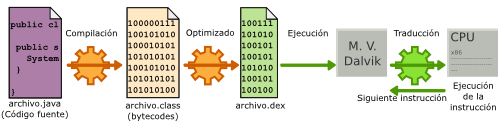
\includegraphics[scale=0.8]{./Android/imagenes/maquinaVirtualDalvik.png}
  \caption{Proceso de ejecución en Android.}
  \label{fig:maquinaVirtualDalvik}
\end{figure}


Los ficheros DEX meten las cadenas duplicadas y las constantes en un mismo fichero para ahorrar espacio, normalmente los archivos DEX suelen ser más pequeños que los archivos JAR de la máquina virtual Java. Una vez instados los archivos DEX pueden ser modificados en el terminal para añadir optimizaciones, reordenado de byte en ciertos datos, quitado de clases vacias, etc. En la versión 2.2 de Android se añadió una nueva característica llamada JIT (Just-In-Time) que es compilación en tiempo real de los archivos DEX, por lo que se pueden añadir nuevas optimizaciones dependiendo de la plataforma.

Todas las aplicaciones de Android se distribuyen en unos archivos con extensión APK. Estos archivos no son más que archivos ZIP con la extensión cambiada. Todos deben tener una estructura idéntica, que se explica a continuación. Contiene diferentes carpetas en las que se incluyen ficheros de configuración, fiecheros necesarios para el funcionamiento de la aplicación y para comprobar la integridad de los mismos.

\begin{itemize}

\item \textbf{META-INF:} en un directorio que contiene tres archivos, \textit{MANIFEST.MF} que es el archivo de manifest, \textit{CERT.RSA} que es el certificado con el que está firmada la aplicación, \textit{CERT.SF} que contiene el hash en SHA-1 de todos los componentes de la aplicación, un ejemplo del archivo \textit{CERT.SF} es el siguiente:

\begin{verbatim}

Signature-Version: 1.0
Created-By: 1.0 (Android)
SHA1-Digest-Manifest: wxqnEAI0UA5nO5QJ8CGMwjkGGWE=
...
Name: res/layout/exchange_component_back_bottom.xml
SHA1-Digest: eACjMjESj7Zkf0cBFTZ0nqWrt7w=
...
Name: res/drawable-hdpi/icon.png
SHA1-Digest: DGEqylP8W0n0iV/ZzBx3MW0WGCA=
\end{verbatim}

\item \textbf{lib:} esta carpeta puede contener otras dependiendo de la plataforma para la que esté diseñada la aplicación. Si por ejemplo tiene código específicamente diseñado para x86 tendrá una carpeta llamada x86, si tiene código para MIPS una llamada mips donde se encontraría el código especialmente diseñado para esta plataforma. Puede que dicha carpeta no exista.

\item \textbf{res:} este directorio contiene todos los recursos que no tienen que ser compilados, como pueden ser imágenes, sonidos, etc.

\end{itemize}

Además de estas carpetas todos los ficheros APK incluyen estos tres archivos.

\begin{itemize}
\item \textbf{AndroidManifest.xml:} es un archivo que sirve para indicar la versión, los permisos que contiene la aplicación, las referencias a librerías, las activitys que contiene la aplicación. En el siguiente listado podemos observar un extracto de los permisos que usamos en la aplicación del proyecto.

\begin{lstlisting}[style=XML]
<uses-permission android:name="android.permission.INTERNET"/>
<uses-permission android:name="android.permission.WRITE_EXTERNAL_STORAGE"/>
<uses-permission android:name="android.permission.WRITE_SETTINGS"/>
<uses-permission android:name="android.permission.GET_ACCOUNTS"/>
<uses-permission android:name="android.permission.USE_CREDENTIALS" />
<uses-permission android:name="android.permission.MANAGE_ACCOUNTS" />
\end{lstlisting}

Podemos ver que con esto garantizamos que la aplicación pueda conectarse a internet, usar la tarjeta SD y manejar las cuentas almacenadas en el móvil, como puede ser la dirección de correo usada para dar de alta el móvil en Google Play.

\item \textbf{classes.dex:} el archivo DEX donde están todas las clases precompiladas en byte code para la máquina virtual Dalvik.

\item \textbf{resources.arsc:} es un fichero que contiene los recursos precompilados como pueden ser los XML de las interfaces de la aplicación, etc.

\end{itemize}

En la imagen~\ref{fig:estructuraAPK} se pueden observar los ficheros y las carpetas comentadas anteriormente del proyecto.

\begin{figure}[h]
  \centering
    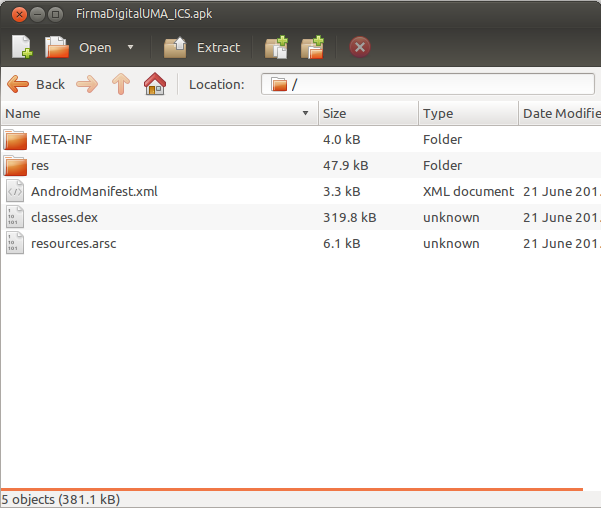
\includegraphics[scale=0.8]{./Android/imagenes/estructuraAPK.png}
  \caption{Estructura del fichero APK del proyecto.}
  \label{fig:estructuraAPK}
\end{figure}

Toda aplicación en Android se construye con unos componentes básicos como pueden ser activities, intents, views, services, contents providers, widgets y un largo etcétera. A continuación vamos a explicar los más importantes.

\begin{itemize}

%poner sección
\item \textbf{Activity:} una activity es la entidad más básica de una interfaz de usuario donde se puede mostrar información en Android, podemos pensar que es como una ventana de cualquier aplicación de escritorio. Cada interfaz que vemos en una aplicación de Android es una activity. Android tiene un ciclo de manejo de activitys bastante complejo, se explicará en la sección~\ref{cap:desarrolandoAndroid} donde pondremos más incapié en el desarrollo de la aplicación móvil del proyecto.

\item \textbf{Intent:} un intent es un componente prácticamente imprescindible en cualquier aplicación de Android, es una forma de comunicación entre cualquier componente. Se pueden definir como mensajes o peticiones, ya que también puede comunicar aplicaciones entre sí. En el proyecto usamos intent para comunicar las activities y poder intercambiar datos entre ellas, también la usamos para abrir el lector de códigos QR que necesitamos, dentro de nuestra aplicación llamamos al intent que nos proporciona la aplicación lectora y cuando termine ella nos devuelve el valor que había en el código QR para que podamos tratarlo.

\item \textbf{View:} son los componentes básicos con los que podemos contruir las interfaces gráficas, como pueden ser botones, barras de texto, campos de texto, spinner, etc. Android pone a nuestra disposición una gran cantidad de estos elementos, y además brinda la posibilidad de crear nuevos, según los vayamos necesitando. Estos objetos normalmente se añaden a una vista y se pueden añadir, modificar o borrar en ella. Estos objetos tienen un ID único en la aplicación por el que podemos controlarlo y añadirle por ejemplo el texto si es un campo de texto o un listener si es un botón para que cuando se pulse realizar la acción que necesitemos.

\item \textbf{Services:} un servicio es un componente de Android que no tiene interfaz gráfica asociada y se ejecuta en segundo plano. Es similar a los servicios que ofrece cualquier sistema operativo. Pueden realizar cualquier acción, tanto recoger o actualizar datos, lanzar notificaciones cada cierto tiempo o mostrar activity para que el usuario introduzca algún valor que necesite.

\item \textbf{Content Provider:} es un mecanismo que posee Android para intercambiar información entre aplicaciones. Por ejemplo cuando usamos la opción de compartir en el teléfono, dentro de una aplicación, nos salen varias aplicaciones con las que podemos compartir directamente, estas son todas las aplicaciones que han implementado el content provider que necesita esta aplicación para compartir la información. En la figura~\ref{fig:contentProvider} podemos ver la opción de compartir de una aplicación y podemos observar como aparece por ejemplo GMail para mandar un email directamente desde aquí sin tener conocimiento de como se produce el intercambio de datos.
 
\begin{figure}[h]
  \centering
    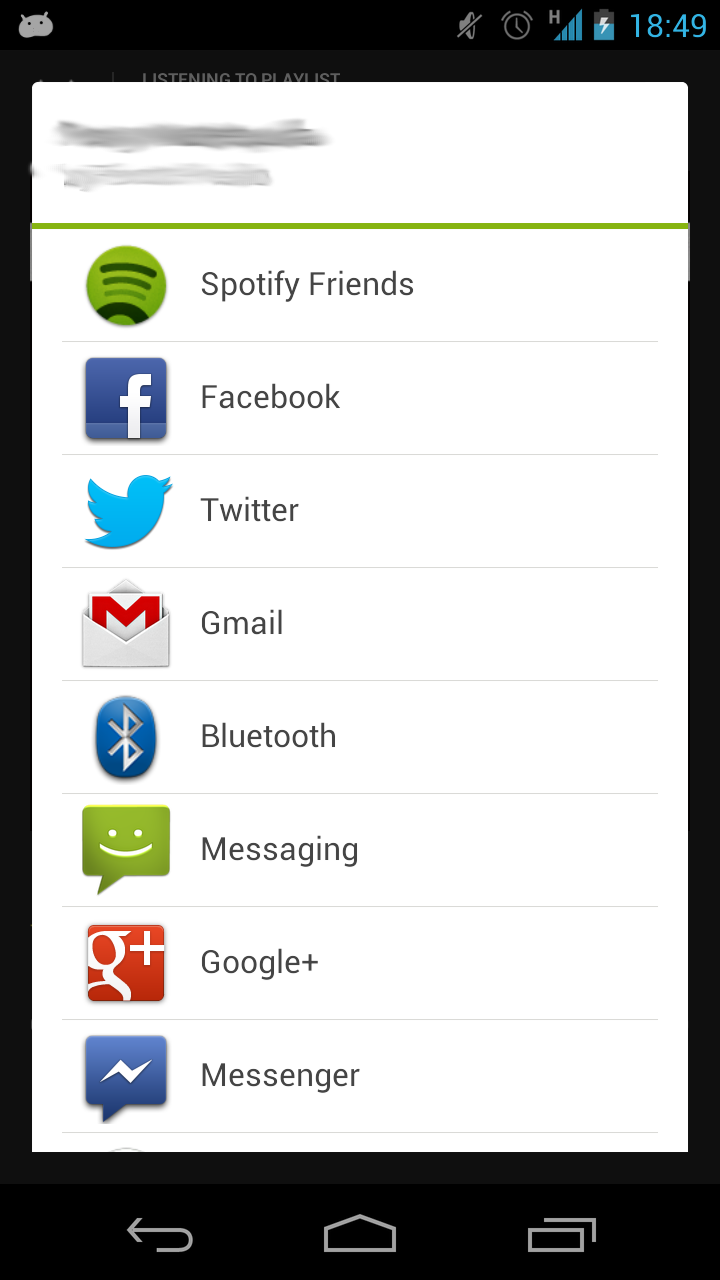
\includegraphics[scale=0.2]{./Android/imagenes/contentProvider.png}
  \caption{Opción compartir de una aplicación.}
  \label{fig:contentProvider}
\end{figure}

\item \textbf{Broadcast Receiver:} es un componente de Android diseñado para actuar cuando ocurre un evento general del sistema, como puede ser la recepción de un SMS, la batería se está agotando, una llamada entrante, etc. También una aplicación puede generar eventos de este tipo para que cualquiera que implemente un Broadcast Receiver pueda recibirlo.

\item \textbf{Widget:} son elementos visuales y generalmente para que el usuario realice alguna acción, tales como poner en pausa la música, pasar de canción, revisar los feed RSS, mirar los correos pendientes, etc. Suele estar en alguna de las pantallas principales de Android. En la figura~\ref{fig:widget} podemos ver un widget de GMail.
 
\begin{figure}[h]
  \centering
    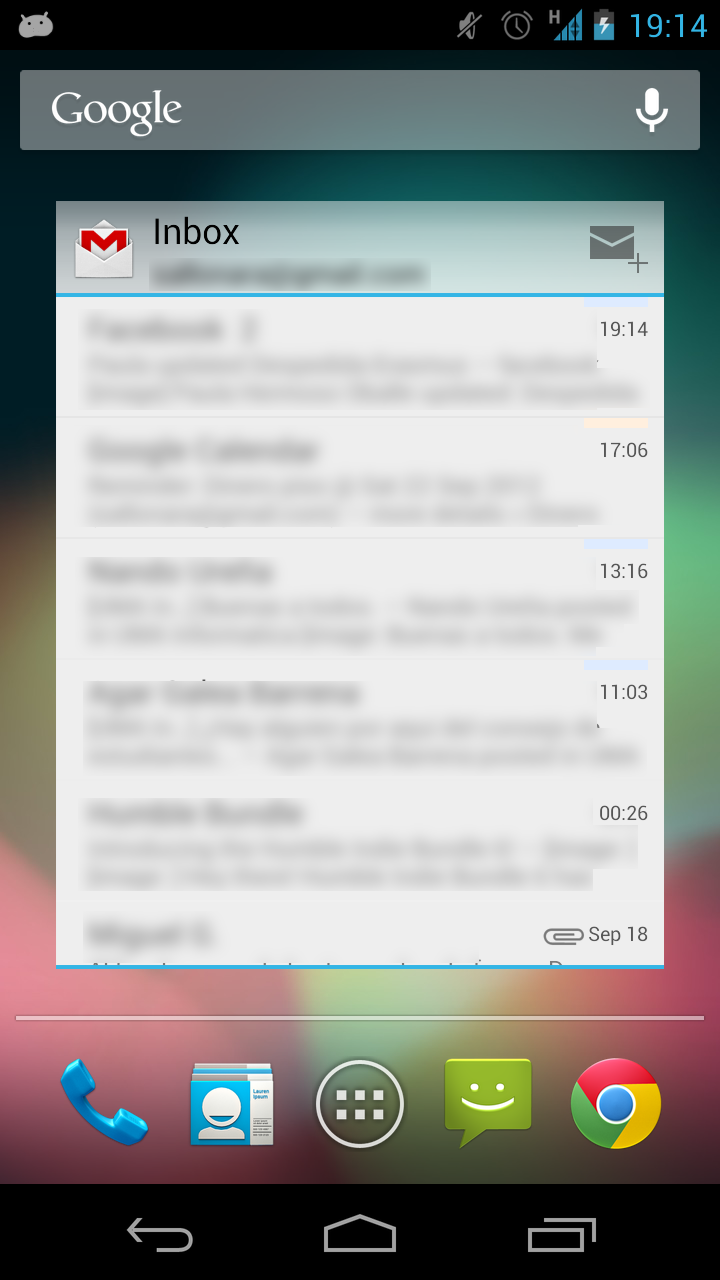
\includegraphics[scale=0.2]{./Android/imagenes/widget.png}
  \caption{Widget de GMail.}
  \label{fig:widget}
\end{figure}

\end{itemize}

\subsection{Desarrollando en Android.}\label{cap:desarrolandoAndroid}

Como ya hemos dicho anteriormente para el desarrollo de la aplicación móvil hemos usado el IDE de programación Eclipse. En el anexo~\ref{cap:apendiceA} podemos ver como realizar la configuración de Eclipse para la programación de aplicaciones Android. En la sección~\ref{cap:proyectoBasico} se explicará con más detenimiento la estructura de un proyecto básico en Android.

En este apartado vamos a explicar las entidades más importantes que existen en Android, como pueden ser las activity, fragment, y view usados en el proyecto.

En el proyecto la entidad más importante que hemos usado es la \lstinline{Activity}. Normalmente las activity están enfocadas a interactuar con el usuario de alguna forma, ya puede ser necesitando de alguna acción del usuario o mostrando información y normalmente ocupan toda la pantalla del terminal, pero puede flotar dentro de otra activity o agruparse con otras usando la clase \lstinline{ActivityGroup}. Todas las subclases que hereden de \lstinline{Activity} tienen que implementar dos métodos imprescindibles. Estos son \lstinline{onCreate(Bundle)} y \lstinline{onPause()}. El primero es donde se inicializa la activity y en el segundo es lo que ocurre cuando el usuario abandona la activity.

Habitualmente toda Activity tiene asociada una interfaz gráfica que se diseña en un fichero XML, como veremos posteriormente, este archivo se le indica a cada Activity con el método \lstinline{setContentView(int);} al cual hay que pasarle una constante que genera automáticamente la clase \lstinline{R} de Android. Una vez se le ha indicado el archivo XML se puede obtener cada uno de los componentes (botones, cuadros de texto, etc) que componen la interfaz gráfica con el método \lstinline{findViewById(int)}. Todo este proceso se tiene que realizar dentro del método \lstinline{onCreate();} y se puede observar en el siguiente trozo de código.

\begin{lstlisting}[style=Java]
@Override
protected void onCreate(Bundle savedInstanceState) {
	super.onCreate(savedInstanceState);
	setContentView(R.layout.initialconfigurescreen);

	TextView tAccountOk = (TextView) findViewById(R.id.tAccountOk);
	EditText tCertificate = (EditText) findViewById(R.id.
		tCertificate);
	ImageView image = (ImageView) findViewById(R.id.imageView1);

	Button bSelectAccount = (Button) findViewById(R.id.bConfigureScreenAccount);
}
\end{lstlisting}

A continuación vamos a explicar las características y su ciclo de vida de las Activity, ya que es un tema muy importante cuando desarrollamos una aplicación Android. En la figura~\ref{fig:cicloActivity} podemos ver todos los estados por los que pasa una Activity desde que se crea hasta que finaliza. 

\begin{figure}
  \centering
    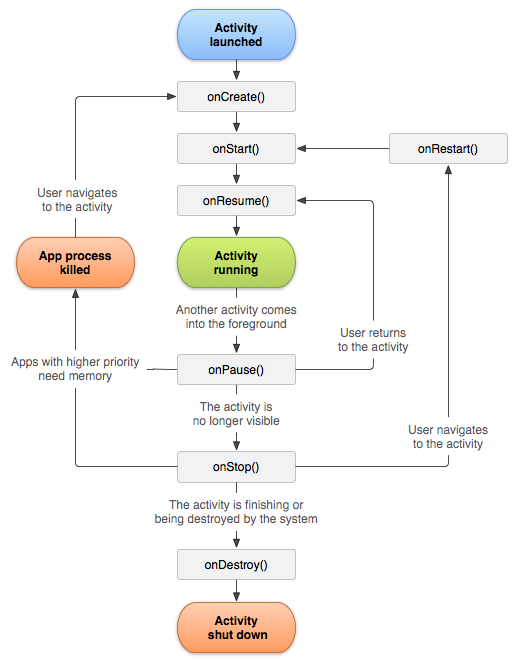
\includegraphics[scale=0.8]{./Android/imagenes/cicloActivity.png}
  \caption{Ciclo de vida de una activity.}
  \label{fig:cicloActivity}
\end{figure}

Todos estos estados se pueden controlar mediante la implementación en la clase que hereda de \lstinline{Activity} de los siguientes métodos.

\begin{lstlisting}[language=Java]
public class Activity extends ApplicationContext {
	protected void onCreate(Bundle savedInstanceState);
	protected void onStart();
	protected void onRestart();
	protected void onResume();
	protected void onPause();
	protected void onStop();
	protected void onDestroy();
}
\end{lstlisting}

Como podemos ver en la figura \ref{fig:cicloActivity} podemos ver que el ciclo completo de una activity es desde el método \lstinline{onCreate(Bundle);} hasta que se realiza la llamada al método \lstinline{onDestroy();}. Como hemos visto antes en \lstinline{onCreate(Bundle);} se genera todo lo necesario para que la activity funcione, como puede ser la inicialización de la interfaz, la creación de un hilo para que realice una operación en background o cualquier otra acción que necesite ser inicializada. El método \lstinline{onDestroy();} se pararía el hilo y se libera la memoria usada por la activity. Entre los procesos \lstinline{onStart();} y \lstinline{onStop();} es donde se mantienen los recursos para que la activity pueda mostrar los datos al usuario. Por ejemplo si tenemos un \lstinline{BroadcastReceiver}, que nos puede cambiar la interfaz de usuario pues lo registramos en el método \lstinline{onStart();} y lo paramos en \lstinline{onStop();}. Estos dos métodos se llaman mucho a lo largo de la ejecución de la activity cada vez que el usuario oculta la activity y vuelve a ejecutarla. Los métodos \lstinline{onResume();} y \lstinline{onPause();} se usan para intercambio de activity, cuando apagamos la pantalla del móvil y volvemos a encenderla, cuando giramos la pantalla, etc. En estos métodos se suelen usar \lstinline{Bundle} para intercambiar información entre los estados y así conseguir por ejemplo restaurar el texto de un cuadro de texto cuando vuelve a generarse.

En esta tabla podemos observar en cada estado del ciclo de vida de una activity puede ser matada y cual sería el próximo estado.
\begin{center}
\begin{tabular}{|l | c | r|}

\hline
Method & ¿Terminable? & Proximo estado\\
\hline
onCreate() & No & onStart()\\
\hline
onRestart() & No & onStart()\\
\hline
onStart() & No & onResume() o onStop()\\
\hline
onResume() & No & onPause()\\
\hline
onPause() & No  & onResume() o onStop()\\
\hline
onStop() & Sí & onRestart() o onDestroy()\\
\hline
onDestroy() & Sí & Ninguna\\
\hline

\end{tabular}
\end{center}

Antes de la versión 3.0 de Android las activity tenían que ocupar toda la ventana y para cambiar o mostrar otra pantalla había que generar una nueva activity de la siguiente forma:

\begin{lstlisting}[style=Java]
Intent intent = new Intent(activity, SplashScreenActivity.class);
startActivity(intent);
\end{lstlisting}

Ese trozo de código se ejecuta en una activity y podemos ver que se crea un objeto \lstinline{Intent} al cual se le dice la activity en la que está y la activity que tiene que iniciar, en este caso la variable \lstinline{activity} es la actual, y \lstinline{SplashScreenActivity} es una activity que tiene la función de inciar todas las variables y realizar las conexiones básicas en el proyecto, acto seguido se usa el procedimiento \lstinline{startActivity(intent);} al que se le pasa el objeto \lstinline{Intent} creado anteriormente y con esto tendríamos la nueva activity ejecutándose.

Desde la versión 3.0 y posteriores las activity siguen ocupando toda la pantalla pero se dio la posibilidad al programador de que usara solo trozos de ella con una clase llamada \lstinline{Fragment} de esta forma no tendría que iniciar una nueva activity cada vez que quiera modificar la interfaz, de este modo se pudieron empezar a usar gestos de scroll laterar para mostrar varias interfaces o en pantallas grandes como una tablet poder modificarla sin tener que generar una nueva activity. 
\begin{figure}
  \centering
    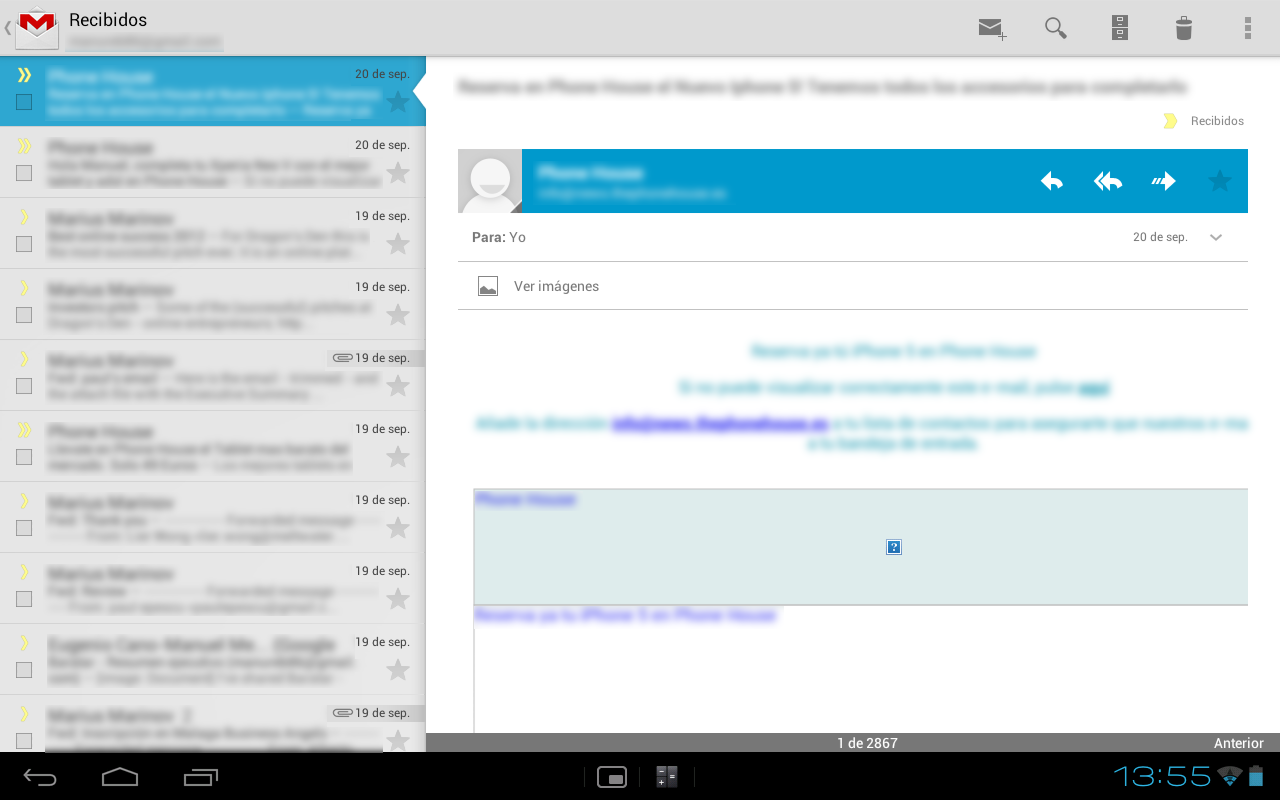
\includegraphics[scale=0.3]{./Android/imagenes/gmailTablet.png}
  \caption{Aplicación de Gmail para tablet.}
  \label{fig:gmailTablet}
\end{figure}

\begin{figure}
  \centering
    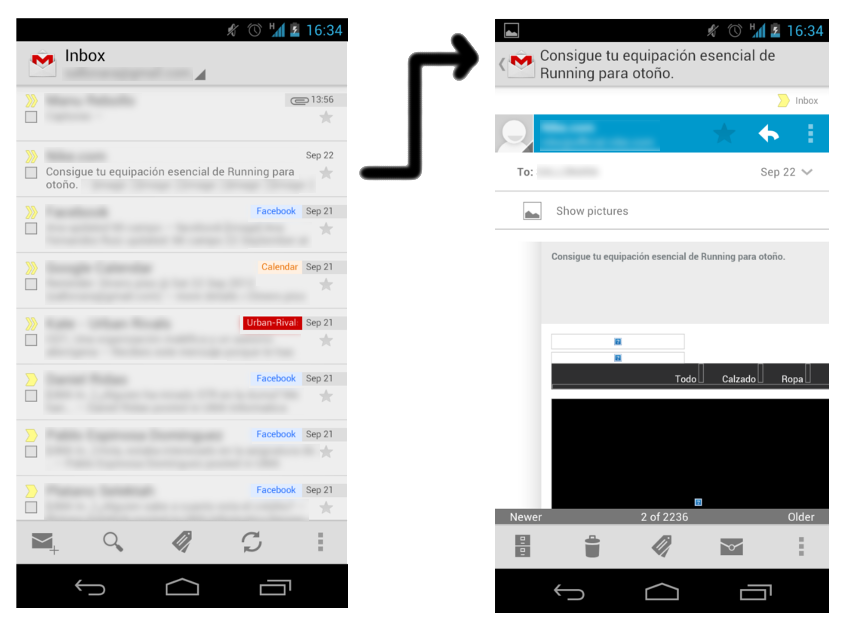
\includegraphics[scale=0.4]{./Android/imagenes/gmailMovil.png}
  \caption{Aplicación de Gmail para móvil.}
  \label{fig:gmailMovil}
\end{figure}

\begin{figure}[h]
  \centering
    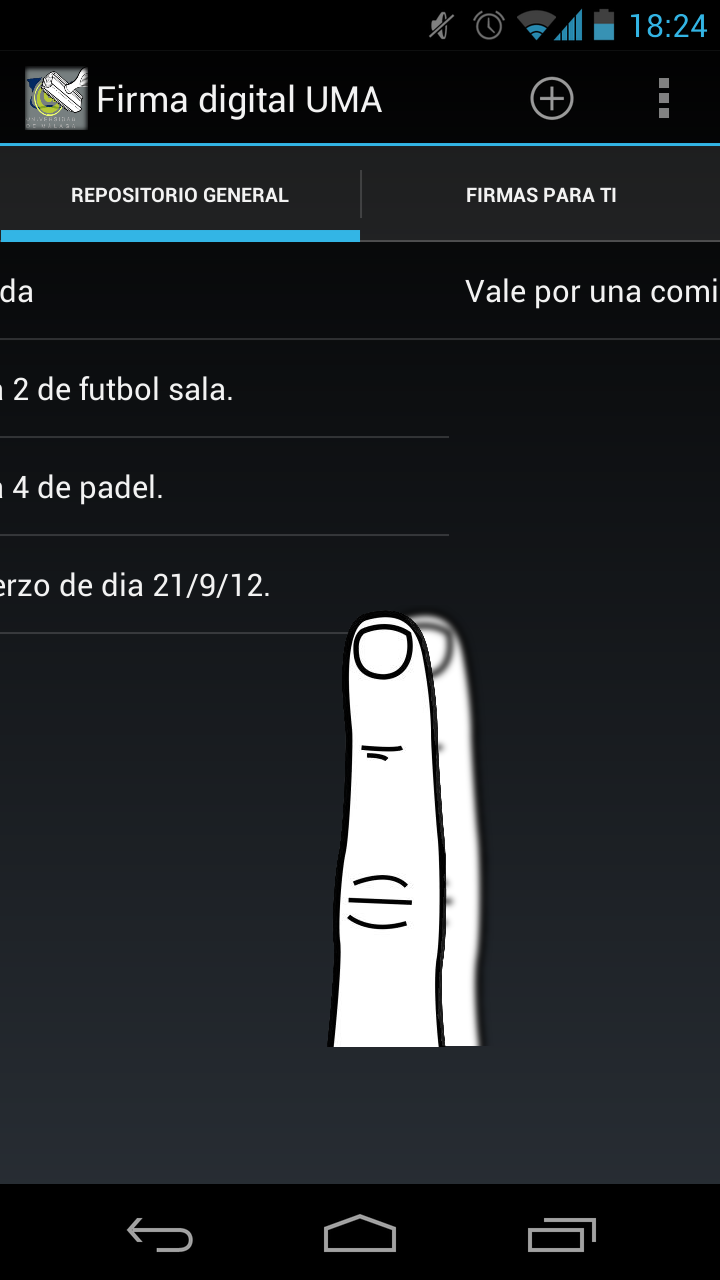
\includegraphics[scale=0.2]{./Android/imagenes/swype.png}
  \caption{Gesto Swype en la aplicación móvil.}
  \label{fig:swype}
\end{figure}

En la imagen~\ref{fig:gmailTablet} podemos ver la aplicación de Gmail diseñada mediante fragment y en ella si pulsamos algún correo en la parte izquierda de la aplicación nos mostraría el correo en la derecha sin tener que recargar la aplicación. En la imagen~\ref{fig:gmailMovil} podemos ver como en la versión movil no se usa esta forma por falta de espacio en la pantalla. Nosotros hemos realizado un diseño para intercambio de fragment mediante un gesto llamado swype o scroll lateral y como se puede ver en la imagen~\ref{fig:swype} podemos ver que no hay que volver a cargar otra activity ni nada, por lo que dotamos a la aplicación de una mayor fluidez.

Para que una aplicación pueda usar una determinada activity, el programador primeramente tiene que definir el uso y su función en el archivo \textit{AndroidManifest.xml}. Podemos ver un extracto de dicho archivo donde definimos un par de activity usadas en el proyecto.
\newpage
\begin{lstlisting}[style=XML]
<activity android:name=".FirmaDigitalUMA_ICSActivity" />
<activity android:name=".InitialConfiguration" android:noHistory=
	"true" />
\end{lstlisting}

Se puede observar que hemos declarado dos activities una sin ninguna opción y otra en la que no se guardará en la pila de llamadas de activity, por lo que si pulsamos el botón atrás no se abrirá de nuevo. Si no realizamos este proceso nos dará un error en tiempo de ejución la aplicación diciendo que hemos intentado ejecutar una activity que no está declarada.

\subsection{Un Proyecto básico de Android en Eclipse.}\label{cap:proyectoBasico}

A continuación vamos explicar con más detenimiento la estructura que tiene un proyecto básico de Android en Eclipse.

\begin{figure}
  \centering
    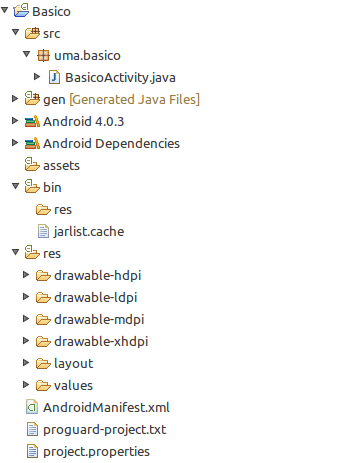
\includegraphics[scale=1]{./Android/imagenes/estructuraBasicaAndroid.png}
  \caption{Estructura básica de un proyecto Android.}
  \label{fig:estructuraBasicaAndroid}
\end{figure}

En la figura~\ref{fig:estructuraBasicaAndroid} podemos ver una captura de un proyecto recién creado. Podemos observar que se genera una carpeta principal en la que posteriormente colgarán el resto de carpetas necesarias. Estas carpetas son \textit{src}, \textit{gen}, \textit{assets}, \textit{bin}, \textit{res} y varios archivos sueltos como con \textit{AndroidManifest.xml}, \textit{proguard-project.txt}, \textit{project.properties}, vamos a explicar brevemente que contiene y cual es la función de dichas carpetas y documentos.

\begin{itemize}

\item \textbf{src:} en esta carpeta están todos los paquetes que contiene los archivos de código fuente que se necesitan en el proyecto.

\item \textbf{gen:} esta carpeta es donde se almacena todo lo que el proyecto de Android necesita para funcionar, casi todos los ficheros que se encuentran en el interior se generan cada vez que se construye el proyecto y si los modificamos nosotros, cuando volvamos a construir el proyecto borrarán los cambios. Dentro está la clase \lstinline{R} donde se declaran la mayoría de las constantes con direcciones de memoria que luego en tiempo de ejecución se usarán para realizar la conversión en bytecode del archivo java.

\item \textbf{bin:} es una carpeta donde se almacenan todos los archivos binarios, como puede ser el archivo APK, los archivos DEX, etc.

\item \textbf{res:} esta carpeta la encargada de contener todos los recursos necesarios para nuestra aplicación. Esta carpeta se divide en varias, como por ejemplo \textit{drawable-hdpi}, \textit{drawable-ldpi}, \textit{drawable-mdpi}, \textit{drawable-xhdpi} es donde se añaden todas imágenes usadas, sonidos, vídeos, etc. Pero no todos los recursos son contenido multimedia, hay otras carpetas como por ejemplo la carpeta \textit{layout} donde se almacenan las diferentes interfaces usadas en el formato XML o la carpeta \textit{values} donde se guardan todas las cadenas constantes en un archivo XML.

\item \textbf{AndroidManifest.xml:} como ya hemos explicado anteriormente es el archivo donde se declara todos los permisos e información de interés de la aplicación, como pueden ser las activity, los intent, la versión mínima que tiene que tener el móvil para ejecutar nuestra aplicación, etc.  

\item \textbf{project.properties:} es un archivo donde se pueden configurar diferentes parámetros del proyecto, como puede ser la API sobre la que se va a ejecutar el proyecto, o si queremos usar una herramienta que ofrece Google dentro del SDK para ofuscar el código llamada ProGuard.

\item \textbf{proguard-project.txt:} ProGuard como hemos dicho antes es una herramienta que ofrece Google dentro del SDK de Android para ofuscación de código, ya que hay muchas herramientas de ingeniería inversa que mediante la decompilación de los archivos DEX se puede llegar casi a conseguir el código realizado sin permiso. En este archivo se puede configurar los diferentes valores para el uso de esta herramienta, tales como son: qué tipo de ofuscación queremos utilizar si solo sintáctica o semántica, si queremos que se pueda tracear la salida del archivo, etc. Para ampliar conocimientos sobre dicha herramienta podemos visitar esta web, \url{http://developer.android.com/tools/help/proguard.html} donde está toda la información necesaria.

\end{itemize}

%-----------------------------------------
%Google App Egine
%-----------------------------------------


\section{Google App Engine.}\label{cap:GAE}
En este apartado de la memoria vamos a explicar lo que es, la configuración y como usar la plataforma Google App Engine.

\subsection{Introducción.}
Google App Engine es una conjunto de APIS que proporciona Google para construir tus propias aplicaciones web, que pueden ser alojadas y usadas en su servicio Google App y vendidas en Google Apps Marketplace. Además de alojamiento gratuito, Google ofrece un dominio, que es como el siguiente: \url{http://nombre\_de\_la\_aplicacion.appspot.com} y una base de datos propietaria de Google que se accede transparentemente a través de su API, gestión de usuarios mediante autentificación con cuentas Google del tipo: usuario@gmail.com, autentificación por federación o openID.

Además de todas estas características Google proporciona APIS para el desarrollo con Java, Python y Go, este último un lenguaje experimental propiedad de Google. Para usar dicha API, Google también proporciona un plugins para Eclipse, en caso de que el lenguaje elegido sea Java, que ayuda al despliegue de la aplicación web, auto completado y gestión de de las aplicaciones creadas. 

En el anexo~\ref{cap:configuracionGAEEclipse} se puede ver como instalar el plugins de Google App Engine para Eclipse.

En el proyecto se ha usado Java, por lo que las APIS de Python y Go no se han estudiado.

En general el uso de Google App Engine para desarrollar aplicaciones web es idéntico a crear una aplicación web con Java 2 Enterprise Edition (Java2EE), se pueden desarrollar servlet que recogen valores mediante métodos \lstinline{GET} o \lstinline{POST} y usar clases Java para hacer operaciones con ellos. A su vez para mostrar la información se pueden generar archivos *.jsp, que son archivos HTML con bloques o líneas de código Java incrustadas, que se introducen con estas etiquetas: \lstinline{<\%= linea de codigo Java \%>} o \lstinline{<\% bloque de codigo Java \%>}. A parte de archivos *.java y *.jsp, debemos tener una carpeta llamada war en la que tiene que ir toda la información de la aplicación web que queremos desplegar. En dicha carpeta hay varias subcarpetas como pueden ser css en la que tiene que ir el estilo de la web o WEB-INF en la que están todos los archivos de configuración, como pueden ser los permisos que tenemos que tener para poder acceder al uso de un servlet, si la web tiene conexión https, la configuración de la base de datos, etc. Más adelante se explicará con más detenimiento todas las carpetas de las que se compone un proyecto de Google App Engine.

Para este proyecto hemos tenido que desarrollar dos aplicaciones web, una que es un servidor de timestamp y otra que es una aplicación para gestión de las firmas digitales que realice cada usuario. A continuación vamos a explicar en profundidad la tecnología usada.

\subsection[Aplicación web genérica en GAE]{Explicación de una aplicación web genérica en Google App Engine.}
En esta parte voy a explicar en profundidad que es un servlet, los archivos de configuración, los archivos JSP y el resto de archivos necesarios para poder desplegar una aplicación en Google App Engine.
 
\subsubsection{¿Qué es un servlet?.}
Un servlet es la evolución de los antiguos applets de Java, su uso más común es generar páginas web dinámicamente con los parámetros que recibe mediante una petición realizada por el navegador web y datos que están almacenados en el servidor web.

Un servlet es un objeto Java que tiene que ser ejecutado en un servidor web o contenedor J2EE, que recibe unos parámetros, realiza una o varias acciones y devuelve un resultado que puede ser desde un código HTML, un JSP que genera dinámicamente un código HTML, un JSON o una simple cadena de texto.

Los servlets, junto con JSP, son la solución de Oracle a la generación de contenido dinámico equivalente al lenguaje PHP, ASP de Microsoft, Ruby, etc.

Los servlets forman parte de Java 2 Enterprise Edition (J2EE) que a su vez es una amplicación de Java 2 Standard Edition (J2SE), para su uso es necesario un servidor web que pueda interpretar código Java, el más famoso es Apache Tomcat que está desarrollado y mantenido por Apache Foundation, que son los encargados también de mantener y desarrollar el famoso servidor web Apache, aunque existen otro como JBoss, Jetty o GlassFish, pero como podremos ver no son los únicos, ya que el propio Google App Engine también funciona internamente a base de servlets y JSP.

Para crear un servlet hay que generar una clase Java que implemente la interfaz \lstinline{javax.servlet.Servlet} como puede ser \lstinline{javax.servlet.http.HttpServlet} que es un servlet específico para conexiones HTTP.
 
Una vez generada la clase hay que implementar el método \lstinline{doGet} para peticiones tipo \lstinline{GET} o el método \lstinline{doPost} para peticiones de tipo \lstinline{POST}. En el siguiente trozo de código se puede ver la implementación más básica de los métodos \lstinline{doGet} y \lstinline{doPost}.

\begin{lstlisting}[style=Java] 
@Override
protected void doGet(HttpServletRequest req, 
	HttpServletResponse resp) throws ServletException, IOException {
	// TODO Auto-generated method stub
	super.doGet(req, resp);
}

@Override
protected void doPost(HttpServletRequest req, 
HttpServletResponse resp) throws ServletException, IOException {
	// TODO Auto-generated method stub
	super.doPost(req, resp);
}
\end{lstlisting}

Una vez implementados los métodos que se necesiten se pueden usar el parámetro \lstinline{HttpServletRequest req} para recibir los valores que queramos enviar a la aplicación web y podemos usar \lstinline{HttpServletResponse resp} para enviar lo que queramos desde una redirección a un JSP, una página web, un JSON o una cadena de texto. 

Un ejemplo de como se reciben los parámetros sería: 

\begin{lstlisting}[style=Java]  
String num_sec = req.getParameter("sec");
\end{lstlisting}

Y si queremos devolver algo, por ejemplo un objeto \lstinline{JSONArray}:

\begin{lstlisting}[style=Java]   
PrintWriter out = resp.getWriter();
out.print(jsonArray);
out.flush();
\end{lstlisting}

Como podemos ver el objeto \lstinline{resp} nos da la posibilidad de conseguir un objeto \lstinline{java.io.PrintWriter} por el que podemos enviar lo que necesitemos.

La forma de acceder a un servlet mandándole peticiones \lstinline{GET} sería la siguiente: \url{https://servertimestamp.appspot.com/search?id=63&texto=Prueba}. Como podemos ver la dirección base es: \url{https://servertimestamp.appspot.com/}, el servlets estaría mapeado internamente en el servidor web, como ya veremos, en la dirección \url{/search} y el primer parámetro va precedido de \url{?id\_parametro} y el resto de \url{\&id\_parametro}. En nuestro ejemplo tendría dos parámetros que son \textit{id} y \textit{texto}, con sus valores después del =.

El método \lstinline{POST} es el utilizado para pasar parámetros por medio de formularios.

\subsection{¿Qué es JSP?.}
JSP es el acrónimo de JavaServer Pages y es una tecnología que ayuda a crear dinámicamente páginas web basadas en HTML o XML y es la solución equivalente a PHP de Oracle. En la figura~\ref{fig:modoJSP} podemos ver el proceso que se hace desde que se realiza la petición en el navegador hasta que se muestra un resultado.

\begin{figure}
  \centering
    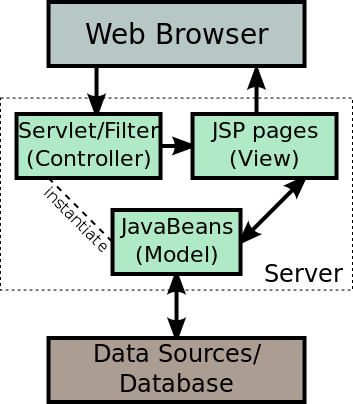
\includegraphics[scale=0.5]{./GoogleAppEngine/imagenes/JSP_Model.png}
  \caption{Modo de interpretación de un archivo JSP}
  \label{fig:modoJSP}
\end{figure}

Un fichero JSP es la unión de código HTML con código Java, el cual es interpretado en el momento de la visualización de la página web. Un ejemplo es el siguiente:
 
\begin{lstlisting}[style=HTML]   
<!DOCTYPE html>
<html>
<body>
<table>
<tr>
	<th>ID</th>
	<th>Num sec</th>
	<th>Token de tiempo</th>
	<th>Mensaje</th>
	<th>URL para ver la firma</th>
	<th>Fecha</th>
	<th>Usuario</th>
	<th id="filadestino">Destino</th>
	<th>Verificado?</th>
</tr>
<% for (RowRepositorioGeneral row : rows) {%>
<tr>
	<td><%=row.getId()%></td>
	<td><%= row.getNum_sec()%></td>
	<td><%=row.getToken_tiempo()%></td>
	<td><%=row.getTexto_claro()%></td>
	<td><a href=<%=row.getUrl_firma()%>>URL para ver el token
			de tiempo</a></td>
	<td><%=row.getFecha()%></td>
	<td><%=row.getUsuario()%></td>
	<td id="filadestino"><%=row.getDestino()%></td>
	<td>
		<%Boolean confirmado = row.getConfirmado();
		if (!(confirmado == null) && confirmado)  else  %>
	</td>
</tr>
<%}%>
</table>
</body>
</html>
\end{lstlisting}

Como se puede ver en este trozo de código de este archivo JSP genera una tabla que se rellena dinámicamente con los valores que devuelve un objeto Java, se puede observar que se entrelazan trozos de código Java con etiquetas HTML. Si mostramos esta web y acto seguido introducimos otro objeto \lstinline{RowRepositorioGeneral} en la estructura, cuando recarguemos la tabla tendrá una fila nueva.

\subsubsection{La carpeta WAR.}

La carpeta WAR es la carpeta principal para el despliegue de una aplicación web, ya que en ella es donde se almacenan todos los archivos que se necesitan para el funcionamiento de la aplicación web, como pueden ser archivos HTML, CSS, JSP, imágenes, etc. En la figura~\ref{fig:carpetawar} se puede observar la carpeta WAR de una de las aplicaciones web realizadas.

\begin{figure}
  \centering
    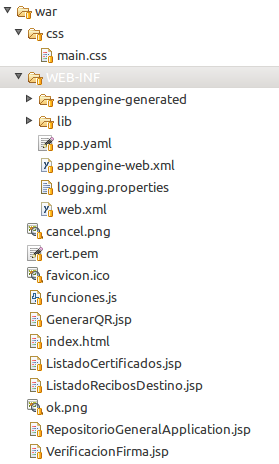
\includegraphics{./GoogleAppEngine/imagenes/carpetawar.png}
  \caption{Carpeta WAR}
  \label{fig:carpetawar}
\end{figure}

Se puede observar las diferentes carpetas y ficheros que la forman. Podemos ver que la carpeta css contiene los archivos de estilo que la página web usará, también podemos ver los archivos web.xml y app.yalm, que son archivos de configuración del servidor que se verán en el próximo apartado~\ref{cap:refArchivosConfiguracionGoogleAppEngine} y además los archivos JSP que se usan en la aplicación junto con los archivos HTML y JavaScript que se necesiten.

\subsubsection{Archivos de configuración.\label{cap:refArchivosConfiguracionGoogleAppEngine}}
Los principales archivos de configuración son web.xml y app.yalm, este segundo es solo una forma de escribir de forma más legible XML, para que nos sea más sencillo entenderlo.

Un ejemplo de un archivo web.xml es el siguiente:

\begin{lstlisting}[language=XML]
<?xml version="1.0" encoding="utf-8"?>
<web-app xmlns:xsi="http://www.w3.org/2001/XMLSchema-
	instance"
xmlns="http://java.sun.com/xml/ns/javaee"
xmlns:web="http://java.sun.com/xml/ns/javaee/web-app_2_5.xsd"
xsi:schemaLocation="http://java.sun.com/xml/ns/javaee
http://java.sun.com/xml/ns/javaee/web-app_2_5.xsd" version=
	"2.5">

	<servlet>
		<servlet-name>AddRow</servlet-name>
		<servlet-class>pfc.ServletCreateRow</servlet-class>
	</servlet>
	<servlet-mapping>
		<servlet-name>AddRow</servlet-name>
		<url-pattern>/add</url-pattern>
	</servlet-mapping>

	<welcome-file-list>
		<welcome-file>ServerTimestampApplication.jsp</welcome-file>
	</welcome-file-list>
</web-app>
\end{lstlisting}

Como se puede observar en el código anterior se ha definido un servlet que se llamará \lstinline{AddRow} que usará la clase \lstinline{ServletCreateRow} y que estará mapeado en la dirección web \url{/add}, también podemos observar que el fichero que nos mostrará el servidor será \lstinline{ServerTimestampApplication.jsp} si entramos a la url principal.

A continuación podemos ver el aspecto de un archivo app.yalm:

\begin{lstlisting}[style=YAML]
application: repositoriorecibos
version: 1
runtime: java

handlers:
  - url: /add
    servlet: pfc.ServletCreateRow
    secure: always
welcome_files:
  - RepositorioGeneralApplication.jsp
\end{lstlisting}

Como podemos observar es mucho más fácil de entender y de escribir, el único problema que tienen los archivos YALM es que son sensibles a los espacios en blanco y tabulaciones, por lo que hay que tener cuidado a la hora de redactarlos. En este archivo se crea un servlet en la ruta \url{/add}, que es la clase Java \lstinline{ServletCreateRow} del paquete \lstinline{pfc} y que siempre hay que estar registrado en la aplicación para poder acceder a él. También podemos observar el fichero de bienvenida para cuando accedemos a la aplicación web. 

Al tener el archivo app.yalm en la carpeta WEB-INF el parseador de YALM  interpreta dicho archivo y genera automáticamente un archivo web.xml que usará el servidor web para su configuración.

Para ver todas las opciones de configuración que se pueden modificar en app.yalm\footnote{ Parámetros de configuración en el archivo app.yalm, \url{https://developers.google.com/appengine/docs/java/configyaml/}} o en web.xml\footnote{ Parámetros de configuración en el archivo web.xml, \url{https://developers.google.com/appengine/docs/java/config/}} se puede consultar los enlaces que hay en las notas al pie.











